52. \begin{figure}[ht!]
\center{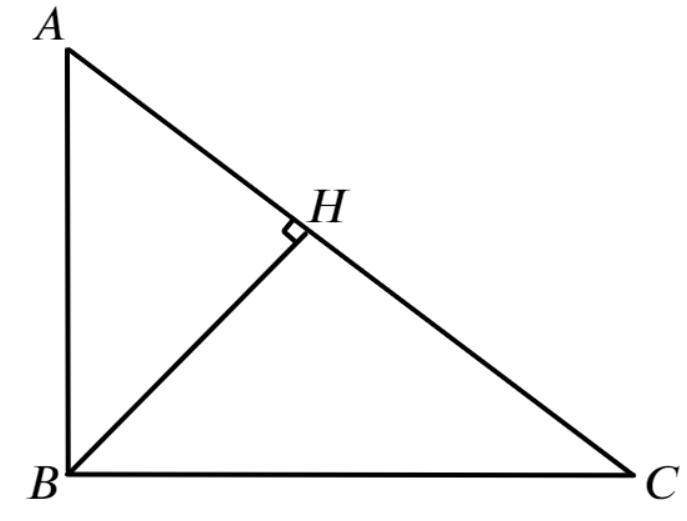
\includegraphics[scale=0.35]{g8-51.png}}
\end{figure}\\
Пусть $AB:AC=3:5,$ тогда $AB=25:5\cdot3=15$см. По теореме Пифагора $BC=\sqrt{625-225}=20$см. Тогда площадь треугольника $ABC$ с одной стороны равна $\cfrac{1}{2}\cdot15\cdot20=150\text{ см}^2,$ а с другой стороны равна $\cfrac{1}{2}BH\cdot25=12,5BH,$ значит $BH=150:12,5=12$см. По теореме Пифагора для треугольника $ABH$ имеем $AH=\sqrt{225-144}=9$см, тогда $HC=25-9=16$см.\\
